\section{3D System Simulation}\label{sec:3d_sim}

\paragraph{}The 2D simulation in the former section serves its purpose as a simple case scenario of the problem. Whereas most of the calculations will be approached in a different way, it follows the same principle.
In this case, the frame will not be a simple cartesian plane, but instead we will consider the WGS84 Geodetic Standard (Section \ref{sec:geodetic}).


\paragraph{} Figure \ref{fig:diagram3D} shows the block diagram used in MATLAB Simulink in order to run this simulation. It is mainly based in the following steps:
\begin{enumerate}
\item{Read Ground Station and Drone GPS position}
\item{Calculate optimal angles (reference), error signal and other parameters. This requires from frames transformation and other functions, and it is performed inside the MATLAB function block, which will be explained later on.}
\item{Input the error signal into the controller.}
\item{Limit the output signal from the controller by the use of the saturation box.}
\item{Input the output signal into Servo-motor model box. This model can be seen in Figure \ref{fig:servomotor3D}, whose parameters have been explain in Chapter \ref{sec:servo_model}.}
\item{Feedback the output angle into the MATLAB function block and repeat again from step 2.}
\end{enumerate}

\begin{figure}[h]
	\centering
	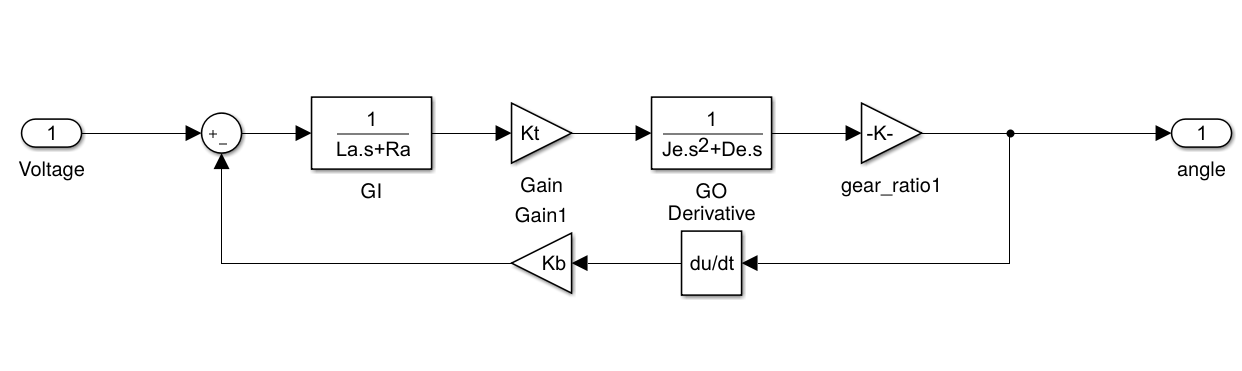
\includegraphics[width=1.1\textwidth]{figures/servomotor_3D.png}
	\caption{Servo-motor Block Diagram}
   	\label{fig:servomotor3D}
\end{figure}

\clearpage

\begin{sidewaysfigure}[h]
	\centering
	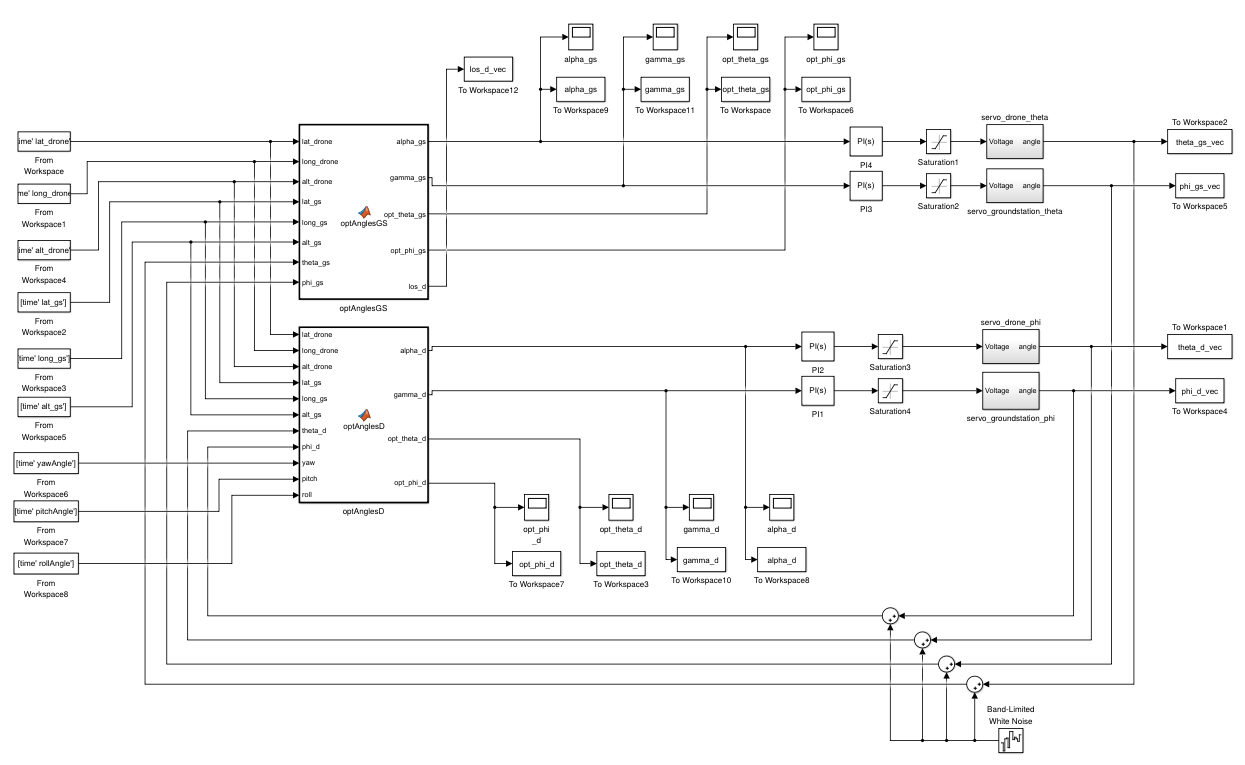
\includegraphics[width=1.1\textwidth,height=1.1\textheight,keepaspectratio]{figures/diagram_3D.png}
	\caption{Block Diagram for 3D Simulation}
   	\label{fig:diagram3D}
\end{sidewaysfigure}

\clearpage

\subsection*{MATLAB Function}
\paragraph{}Firstly note that, as explain in section \ref{sec:opt_angle}, this function is duplicated since almost the same calculations for Ground Station and Drone have to be done, being the only diference the reference (origin) for the local NED transformation.
The Ground station version will transform the Drone GPS coordinates to ECEF and then to the local NED Frame with respect to the Ground Station position. The Drone version do the analgous calculation but the NED Frame will be with respect to the Drone position.
\paragraph{}After this, the \textbf{optimal} or {reference} angles will be calculated according to the equations \ref{eq:OptGS} and the error signal obtained by substracting this calculated angle with the current angle position of the antenna, which comes from the outer loop feedback.

\begin{figure}[h]
	\centering
	\includegraphics[width=1\textwidth]{figures/Map_sim.eps}
	\caption{Map}
   	\label{fig:map}
\end{figure}

\begin{figure}[h]
	\centering
	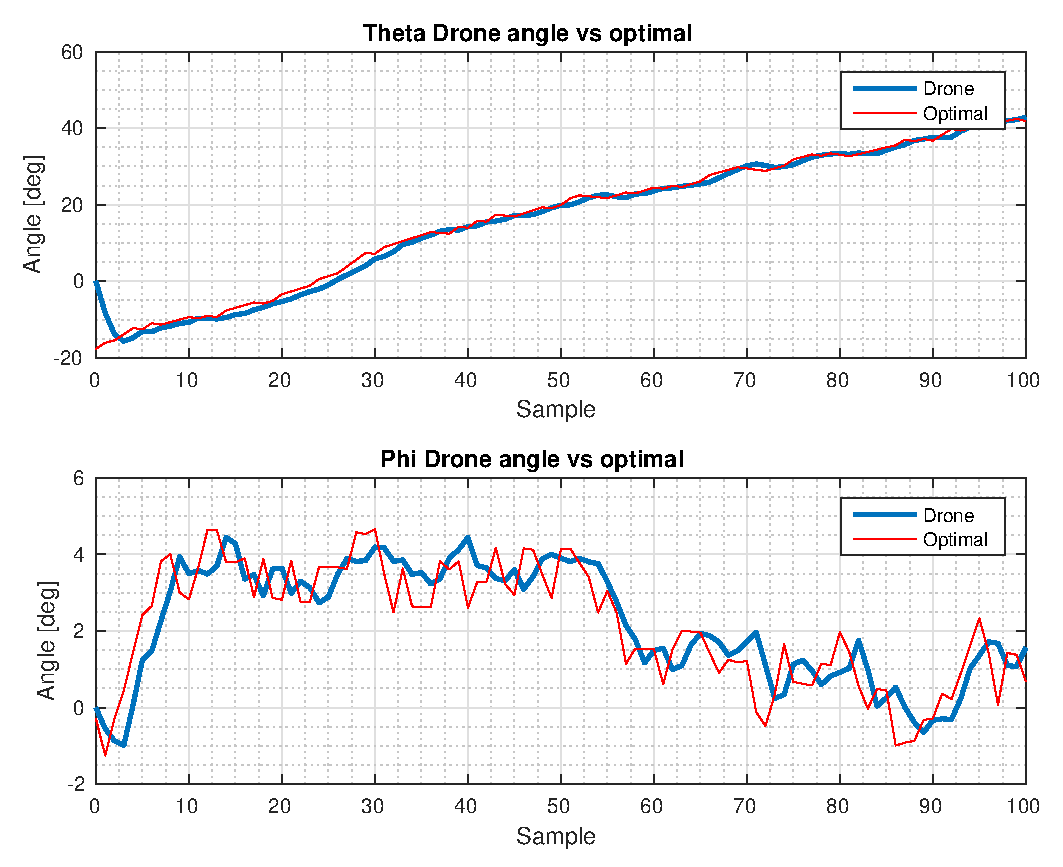
\includegraphics[width=1\textwidth]{figures/Drone_angles.eps}
	\caption{Drone angles}
   	\label{fig:Drone_angles}
\end{figure}

\begin{figure}[h]
	\centering
	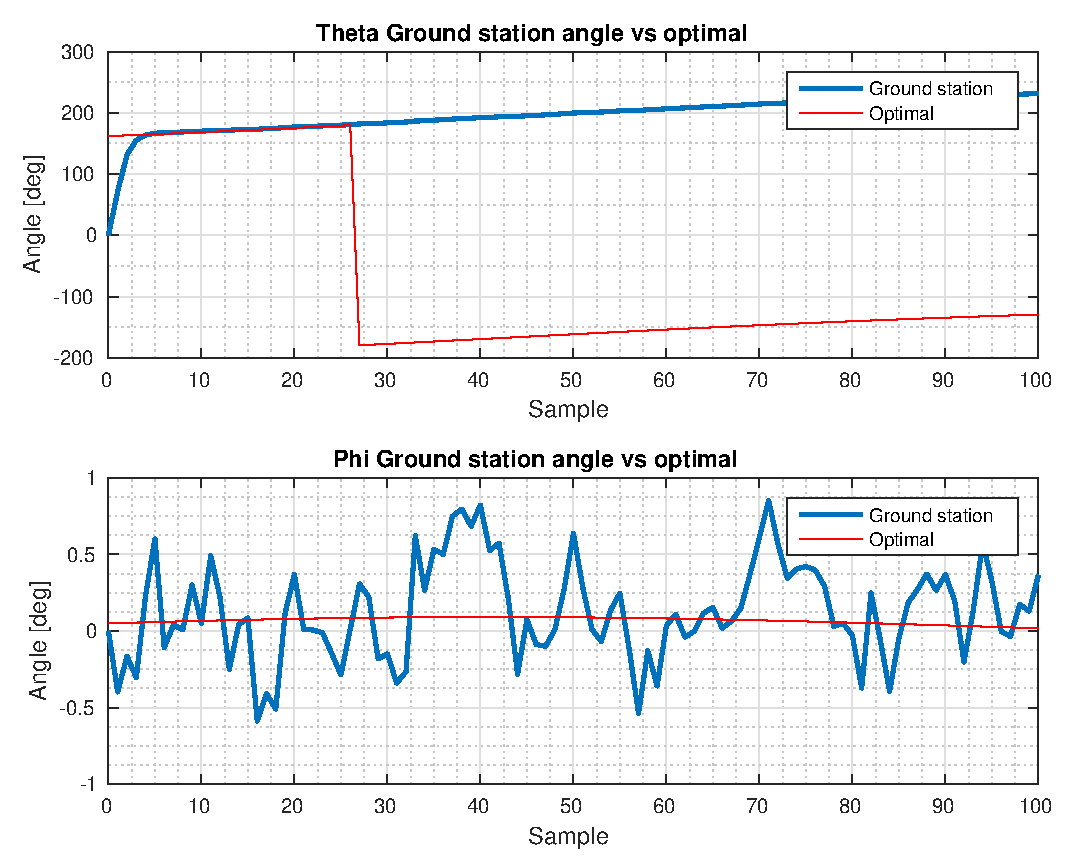
\includegraphics[width=1\textwidth]{figures/GS_angles.eps}
	\caption{Ground Station angles}
   	\label{fig:GS_angles}
\end{figure}